\documentclass[12pt,a4paper]{article}
%-------------------------------------------
%---Packages--------------------------------
%-------------------------------------------
\usepackage[utf8]{inputenc}
%\usepackage[T1]{fontenc}
%\usepackage{txfonts}
\usepackage{amsmath}
\usepackage{amsthm}
\usepackage{amsfonts}
\usepackage{array}
\usepackage{amssymb}
\usepackage{blindtext}
\usepackage{caption}
\usepackage{color}
\usepackage{csquotes}	    %
\usepackage{enumitem}	    %pour mieux bosser avec les listes. ajoute option label
\usepackage[yyyymmdd]{datetime}        %pour définir date custom
\usepackage{etaremune}
\usepackage{environ}
\usepackage{fancybox}
\usepackage{fancyhdr} 	    % Custom headers and footers
\usepackage{fancyref}
%\usepackage{float}
\usepackage{floatrow}       %float and floatrow can't be together...
\usepackage{gensymb}
\usepackage{graphicx}
\usepackage[colorlinks=true, linkcolor=purple, citecolor=cyan]{hyperref}
\usepackage{footnotebackref}
\usepackage{lipsum}
\usepackage{mathtools}
\usepackage{multicol}	    %gérer plusieurs colonnes
\usepackage{setspace}
\usepackage{subcaption}
\usepackage{todonotes}	    %Bonne gestion des TODOs
%TODO commenté pour tester l'utilité... à voir% \usepackage[tc]{titlepic}      %Permet de mettre une image en page de garde
\usepackage{tikz}	    % Pour outil de dessin puissant
\usepackage{ulem}	    %underline sur plusieurs lignes (avec \uline{})
\usepackage{vmargin} 	    %gestion des marges, avec dans l'ordre : gauche, haut, droit, bas, en-tête, entre en-tête et texte, bas de page, hauteur entre bas de page et texte
\usepackage{wrapfig}
\usepackage{xcolor}
\usepackage{xparse}                    %Pour utiliser NewDocumentCommand et des arguments 'mmooo'
%\usepackage{fullpage} 	    %supprime toutes les marges allouées aux notes, aussi en haut et en bas

%\ExplSyntaxOn
\pagestyle{fancyplain}	    %Makes all pages in the document conform to the custom headers and footers

%-------------------------------------------
%---Document Commands-----------------------
%---------------------------{----------------
\NewDocumentCommand{\framecolorbox}{oommm}
 {% #1 = width (optional)
  % #2 = inner alignment (optional)
  % #3 = frame color
  % #4 = background color
  % #5 = text
  \IfValueTF{#1}%
   {\IfValueTF{#2}%
    {\fcolorbox{#3}{#4}{\makebox[#1][#2]{#5}}}%
    {\fcolorbox{#3}{#4}{\makebox[#1]{#5}}}%
   }%
   {\fcolorbox{#3}{#4}{#5}}%
 }%
%------------------------------------------------
%------------------ENGLISH----------------------
%----------------------------------------------

\NewDocumentCommand{\epflTitle}{mO{Olivier Cloux}O{\today}O{Notes de Cours en}D<>{../../Common}}%Arguments : Matière, Auteur, Date, Titre du doc
{
\begin{titlepage}
    \vspace*{\fill}
    \begin{center}
        \normalfont \normalsize
        \textsc{Ecole Polytechnique Fédérale de Lausanne} \\ [25pt] % Your university, school and/or department name(s)
        \textsc{#4} %Titre du doc
        \\ [0.4 pt]
        \horrule{0.5pt} \\[0.4cm] % Thin top horizontal rule
        \huge #1 \\ % Matière
        \horrule{2pt} \\[0.5cm] % Thick bottom horizontal rule
        
\includegraphics[width=8cm]{#5/EPFL_logo}
        ~\\[0.5 cm]
        \small\textsc{#2}\\[0.4cm]
        \small\textsc{#3}\\
        ~\\
        ~\\
        
\includegraphics[scale=0.5]{#5/creativeCommons}
    \end{center}
    \vspace*{\fill}
\end{titlepage}
}


%-------------------------------------------
%-------------MATH NEW COMMANDS-------------
%-------------------------------------------
\newcommand{\somme}[2]{\ensuremath{\sum\limits_{#2}^{#1}}}
\newcommand{\produit}[2]{\ensuremath{\prod\limits_{#2}^{#1}}}
\newcommand{\limite}{\lim\limits_}
\newcommand{\llimite}[3]{\limite{\substack{#1 \\ #2}}\left(#3\right)}	%limites à deux condiitons
\newcommand{\et}{\mbox{ et }}
\newcommand{\deriv}[1]{\ensuremath{\, \mathrm d #1}}	%sigle dx, dt,dy... des dérivées/intégrales
%\newcommand{\fx}{\ensuremath{f'(\textbf{x}_0 + h}}
\newcommand{\ninf}{\ensuremath{n \to \infty}}	       %pour les limites : n tend vers l'infini
\newcommand{\xinf}{\ensuremath{x \to \infty}}	       %pour les limites : x tend vers l'infini
\newcommand{\infint}{\ensuremath{\int_{-\infty}^{\infty}}}
\newcommand{\xo}{\ensuremath{x \to 0}}									%x to 0
\newcommand{\no}{\ensuremath{n \to 0}}									%n zéro
\newcommand{\xx}{\ensuremath{x \to x}}									%x to x
\newcommand{\Xo}{\ensuremath{x_0}}										%x zéro
\newcommand{\X}{\ensuremath{\mathbf{X}} }
\newcommand{\A}{\ensuremath{\mathbf{A}} }
\newcommand{\R}{\ensuremath{\mathbb{R}} }								%ensemble de R
\newcommand{\rn}{\ensuremath{\mathbb{R}^n} } 							%ensemble de R de taille n
\newcommand{\Rm}{\ensuremath{\mathbb{R}^m} }  							%ensemble de R de taille m
\newcommand{\C}{\ensuremath{\mathbb{C}} }
\newcommand{\N}{\ensuremath{\mathbb{N}} }
\newcommand{\Z}{\ensuremath{\mathbb{Z}} }
\newcommand{\Q}{\ensuremath{\mathbb{Q}} }
\newcommand{\rtor}{\ensuremath{\R \to \R} }
\newcommand{\pour}{\mbox{ pour }}
\newcommand{\coss}[1]{\ensuremath{\cos\(#1\)}}						%cosinus avec des parenthèses de bonne taille (genre frac)
\newcommand{\sinn}[1]{\ensuremath{\sin\(#1\)}}					%sinus avec des parentèses de bonne taille (genre frac)
\newcommand{\txtfrac}[2]{\ensuremath{\frac{\text{#1}}{\text{#2}}}}		%Fractions composées de texte
\newcommand{\evalfrac}[3]{\ensuremath{\left.\frac{#1}{#2}\right|_{#3}}}
\renewcommand{\(}{\left(}												%Parenthèse gauche de taille adaptive
\renewcommand{\)}{\right)}
\newcommand{\longeq}{=\joinrel=}												%Parenthèse droite de taille adaptive


%-------------------------------------------------------
%------------------MISC NEW COMMANDS--------------------
%-------------------------------------------------------
\newcommand{\degre}{\ensuremath{^\circ}}
%\newdateformat{\eudate}{\THEYEAR-\twodigit{\THEMONTH}-\twodigit{\THEDAY}}



%-------------------------------------------------------
%------------------TEXT NEW COMMANDS--------------------
%-------------------------------------------------------
\newcommand{\ts}{\textsuperscript}
\newcommand{\evid}[1]{\textbf{\uline{#1}}}        %mise en évidence (gras + souligné)



%\newcommand{\Exemple}{\underline{Exemple}}
\newcommand{\Theoreme}{\underline{Théorème}}
\newcommand{\Remarque}{\underline{Remarque}}
\newcommand{\Definition}{\underline{Définition} }
\newcommand{\skinf}{\sum^{\infty}_{k=0}}
\newcommand{\combi}[2]{\ensuremath{\begin{pmatrix} #1 \\ #2 \end{pmatrix}}}	%combinaison parmi 1 de 2
\newcommand{\intx}[3]{\ensuremath{\int_{#1}^{#2} #3 \deriv{x}}}				%intégrale dx
\newcommand{\intt}[3]{\ensuremath{\int_{#1}^{#2} #3 \deriv{t}}}				%intégrale dy
\newcommand{\misenforme}{\begin{center} Mis en forme jusqu'ici\\ \line(1,0){400}\\ normalement juste, mais à améliorer depuis ici\end{center}}	%raccourci pour mise en forme
\newcommand*\circled[1]{\tikz[baseline=(char.base)]{
            \node[shape=circle,draw,inner sep=1pt] (char) {#1};}}			%pour entourer un chiffre
\newcommand{\horrule}[1]{\rule{\linewidth}{#1}} 				% Create horizontal rule command with 1 argument of height

\theoremstyle{definition}
\newtheorem{exemp}{Exemple}
\newtheorem{examp}{Example}


%-------------------------------------------
%---Environments----------------------------
%-------------------------------------------
\NewEnviron{boite}[1][0.9]{%
	\begin{center}
		\framecolorbox{red}{white}{%
			\begin{minipage}{#1\textwidth}
 	 			\BODY
			\end{minipage}
		}
	\end{center}
}
\NewEnviron{blackbox}[1][0.9]{%
	\begin{center}
		\framecolorbox{black}{white}{%
			\begin{minipage}{#1\textwidth}
 	 			\BODY
			\end{minipage}
		}
	\end{center}
}
\NewEnviron{exemple}[1][0.8]{%
    \begin{center}
        \framecolorbox{white}{gray!20}{%
            \begin{minipage}{#1\textwidth}
                \begin{exemp}
                    \BODY
                \end{exemp}
            \end{minipage}
        }
    \end{center}
}
\NewEnviron{suiteExemple}[1][0.8]{%
    \begin{center}
        \framecolorbox{white}{gray!20}{%
            \begin{minipage}{#1\textwidth}
                \BODY
            \end{minipage}
        }
    \end{center}
}
\NewEnviron{colExemple}[1][0.8]{%
    \begin{center}
        \framecolorbox{white}{gray!20}{%
            \begin{minipage}{#1\columnwidth}
                \begin{exemp}
                    \BODY
                \end{exemp}
            \end{minipage}
        }
    \end{center}
}
\NewEnviron{example}[1][0.8]{%
    \begin{center}
        \framecolorbox{white}{gray!20}{%
            \begin{minipage}{#1\textwidth}
                \begin{examp}
                    \BODY
                \end{examp}
            \end{minipage}
	}
    \end{center}
}
\NewEnviron{systeq}[1][l]{
			\begin{center}
				$\left\{\begin{array}{#1}
					\BODY
				\end{array}\right.$
			\end{center}
 }





%-------------------------------------------
%---General settings-----------------------
%-------------------------------------------
\renewcommand{\headrulewidth}{1pt}										%ligne au haut de chaque page
\renewcommand{\footrulewidth}{1pt}										%ligne au pied de chaque page
\setstretch{1.6}
\author{Olivier Cloux}

\usepackage[tc]{titlepic}
\usepackage{graphicx}
\usepackage{subcaption}
\usepackage{float}
\date{Fall 2015}
\renewcommand{\contentsname}{Table of Contents}

\NewEnviron{code}{
	\begin{center}
		\texttt{
		\BODY
		}
	\end{center}
}
\begin{document}
\setstretch{1}
\epflTitle{Functional Programming}[Olivier Cloux][Fall 2015][Lectures notes in]	%Chose \epflTitleEN{#1}[#2][#3] #1 mand. : course's name, #2 opt. : name, #3 opt. : Date
\tableofcontents
\setstretch{1.3}

\section{Functions \& Evaluations}
\evid{Evaluation} Non-primitive expressions are evaluated as follow :
\begin{enumerate}
	\item  	Take leftmost operator
	\item 	Evaluate it's operand (left before right) 
	\item 	Apply the operator to the operands. 
\end{enumerate}
{For functions, we use the} \textit{substitution model}
\begin{enumerate}
	\item 	Evaluate all functions arguments, from left to right	
	\item 	Replace the function application by the function's right-hand side, and, at the same time
	\item 	replace the formal parameters of the function by the actual arguments
\end{enumerate} 
\evid{Call by name/value :} Let \textit{sumOfSquares(a,b)} be a function that returns the sum of the square of two Int. A \textbf{call by value} would do : \textit{sumOfSquares(3, 2+2), sumOfSquares(3, 4), square(3) + square(4), 3*3 + square(4) ....}, when a \textbf{call by name} would do : \textit{sumofSquares(3, 2+2), square(3) + square(2+2), 3*3 + square(2+2), 9+square(2+2), 9+ (2+2)*(2+2), 9+4*(2+2), 9+4*4, 25}.

Theory says : if CBV terminates, then CBN terminates. Other direction is not true.\\
\evid{val/var/def} \textit{def} is "by-name", it's right-hand side is evaluated on each use. \textit{val} is evaluated at the point of \textit{val} itself and afterwards, the name refers to the value.


\section{High order functions}
Sometimes, we want to create a function that takes functions as parameters. For example, we want to compute the sum of something. But we might want to compute the sum of squares of those Int, cube, factorial of their product,... We could write a function for everything, but writing a higher order function would be more useful.

\begin{figure}[h]
	\centering
	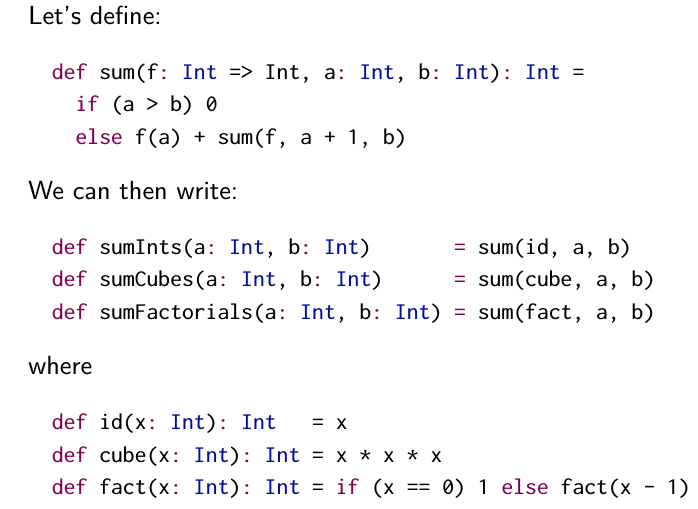
\includegraphics[scale=0.5]{images/sum_HighOrder}
	\caption{Summing with high order functions}
\end{figure}
But this is very tedious. One might prefer to shorten these functions, by not defining them (with \textit{def}), and not precise their type. This is why we "define" \evid{Anonymous functions}. They are functions one can write without giving them a name.
\begin{exemple}
		An anonymous function that raises it's argument to a cube : 
		\begin{code}
			(x: Int) =$>$ x*x*x
		\end{code}
\end{exemple}
Note that the type of the parameter can be omitted  if it can be inferred by the compiler from the context. If there are several parameters, they are separated by commas. Now, using these to write our sum would make it really easier :
\begin{figure}[h]
	\centering
	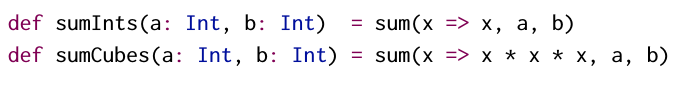
\includegraphics[scale=0.5]{images/sum_Anonymous}
	\caption{Summing with anomymous functions}
\end{figure}

\subsection{Currying}
All functions seen above use the same parameters a and b. We can shorter even more, by getting rid of these parameters. For that, we first shorten our {\tt sum} function, so it returns a new function that will depend on the parameter function :
\begin{verbatim}
	def sum(f: Int => Int): (Int, Int) => Int = {
	   def sumF(a: Int, b: Int): Int =
	      if (a > b) 0
	      else f(a) + sumF(a + 1, b)
	   sumF
	}
\end{verbatim}
Not, the return type of {\tt sum} is a function. The returned function {\tt sumF} applies the given function parameter {\tt f} and sum the results. We can then define :
\begin{verbatim}
	def sumInts = sum(x => x)
	def sumCubes = sum(x => x*x*x)
	def sumFactorials = sum(fact)
\end{verbatim}
But can we avoid the {\tt sumInts},... middlemen ? Yes, with {\tt sum (cube) (1, 10)}. This will apply sum to cubes and return the sum of cubes function. Generally, \uline{function application associates to the left}.

The definition of functions that return functions is so useful in Scala that there is a special syntax for that. We can so reduce our {\tt sum} function to :
\begin{verbatim}
	def sum(f: Int => Int)(a: Int, b: Int): Int =
	   if(a > b) 0   else f(a) + sum(f)(a + 1, b)
\end{verbatim}
So, the very definition of \textbf{currying} is a style of definition ; we can show that 
\begin{code}
	def f(args1)(args2)...(argsN) = E
\end{code}
is equivalent to 
\begin{code}
	def f = (args1 => (args2 => ...(argsN => E)...))
\end{code}
And that is currying.\\
\evid{Type} And now, we can define what is the type of {\tt sum} : {\tt (Int => Int) => (Int => Int) => Int}. We have to note that \textbf{functional types associate to the right}. That is to say that
\begin{center}
	{\tt Int => Int => Int} is equivalent to {\tt Int => (Int => Int)}
\end{center}
\section{Data and Abstraction}
\subsection{Class Hierarchies}
Abstract class 
\section{Week 4}
\section{Lists}
\subsection{Operations/functions}
Given a list of n elements (called xs) and a list ys of m elements, we can use various functions on it : 
\setstretch{1}
\begin{itemize}
	\item 	xs.length : the length (\# of elements) of the list
	\item 	xs.head : the very first element of the list
	\item 	xs.tail : the list except the first element (head)
	\item 	xs.last : the last element of the list.
	\item 	xs.init : the list, except the last element.
	\item 	xs take n : (at most) the n first element of the list
	\item 	xs drop n : the list without the n first elements
	\item 	xs(n) : the element of the list at index n
	\item 	xs ++ ys (or xs ::: ys) : concatenation of the two lists. One list of size n+m.
	\item 	xs.reverse : the same list but in reverse order.
	\item 	xs updated(n,x) : the same list, but with the element at index n replaced by x
	\item 	xs index of x : the index of the element x in xs.
	\item 	xs contains x : a boolean, if the list contains x or not.
	\item	x :: xs : the list xs with x added before the head. (new list of size n+1)
	\item 	xs splitAt n : returns a 2-tuple, first is a list of the n first elements, second is a list of the remaining
\end{itemize}
\setstretch{1.2}
\subsection{Implicit parameters}
You can pass a parameter to a function, adding \texttt{implicit} in front of the parameter. That way, if the type is explicit enough (String, Int,...) the compiler will try and found what you meant (for a comparator, it will find the best comparator with math.Ordering). If you want to use your function on non-explicit types, you can still precise an explicit argument.

\subsection{Reduction of lists}
\subsubsection{reduceLeft}
Given a list xs, you can apply on each element the an operation (like the sum of all elements), either with pattern matching (case x :: xs => x + sum(xs)) or with \textbf{reduceLeft}.
\begin{verbatim}
	List(x1,...,xn) reduceLeft op = (...(x1 op x2) op ... ) op xn
\end{verbatim}
\begin{exemple}~\\
	\texttt{def sum(xs: List[Int]) = \\(0 :: xs) reduceLeft ((x,y ) =$>$ x + y)}\\
	The (0::xs) part is here to avoid the summation of a Nil. It could still add 0 to nothing, and thus have 0.\\
	You can also write \texttt{(0::xs) reduceLeft (\_+\_)}
\end{exemple}

\subsubsection{foldLeft}
Basically the same than reduceLeft, but with an accumulator	as an additional parameter that will be returned when foldLeft is called on an empty list.
\begin{exemple}~\\
\texttt{def sum(xs: List[Int]) = (xs reduceLeft 0)(\_+\_)}
\end{exemple}

\subsection{Reasoning about concat}
We look again at induction. First, \textbf{natural induction} is about simple elements (prove that for $n \geq 4$, $factorial(n) > power(2, n)$). To apply the same principles, we use \textbf{structural induction} (prove a property P(xs) for all lists xs). We first have to prove the base case (P(Nil) and then prove that, if it holds for P(xs), it holds for P(x :: xs) too. Change xs by x::xs in both side of the equation, and try to make them similar.

\section{Collections}
\subsection{Other Collections}
Lists are linear. Access first is super fast, accessing last is super slow. That's why we have \textbf{vectors}. The time to access elements is more balanced. You start as a list. If you have more than 32 elements, each cell becomes a pointer to an other vector (of size max 32). This process can repeats with 6 levels. Operations are similar than with lists. Except, to add an element to the left of the vector you use \texttt{x +: xs}, and to add it to the right you use \texttt{xs :+ x}

\evid{A note about iterables :} Lists and Vectors are both subclasses of Sequence. Sequence (as well as Set and Map) is a subclass of iterable. Array and Strings support the same operations as Seq and can be implicitly converted to sequences. They are not subclasses of Seq, as they come from Java.

\evid{Range :} It is possible to write a range of numbers, with operators \texttt{until}, \texttt{to} and \texttt{by}. 
\begin{exemple}
	\texttt{val r: Range = 1 until 5} is 1,2,3,4\\
	\texttt{val s: Range = 1 to 5} is 1,2,3,4,5\\
	\texttt{1 to 10 by 3} is 1,4,7,10\\
	\texttt{6 to 1 by -2} is 6,4,2
\end{exemple}
Range is also a subclass of Sequence.
\subsubsection{Operations on sequences}
\setstretch{1}
\begin{itemize}
	\item 	xs exists p : true if there is an element x of xs such that p(x) holds, false otherwise
	\item 	xs forall p : true if p(x) holds for all elements x of xs, false otherwise.
	\item 	xs zip ys : a sequence of pairs drawn from corresponding elements of sequence xs and ys. size is size of smallest list ; when one list is empty, remaining elements in the other list are dropped.
	\item 	xs.unzip  : opposite to zip. separates list of pairs into 2 lists (one is first elements, other is second element)
	\item  	xs flatMap f : takes every element in xs, apply the function on them (one at a time) and returns a new list, consisting of the modified elements.
	\item 	xs. product, xs.sum, xs.min, xs.max : if numeric type, product, sum, minimum or maximum of all elements. Max and min also possible if not numeric, but an Ordering must exist.
\end{itemize}
\setstretch{1.2}
\subsection{Combinatorial search and for-expressions}
Given a vector of vectors of tuples, we want to "flatten" it to have only a list of tuples. We simply use \texttt{flatten} to have a list of tuples. Note also that use \texttt{flatten} after a \texttt{map} is equivalent to using \texttt{flatMap}
\subsubsection{For syntax}
The general syntax for a \texttt{for} query is of the form \texttt{for (s) yield e} with e an expression whose value is returned by an iteration, and s is a sequence of \uline{generators} and \uline{filters}. A \uline{generator} is of the form \texttt{p <- e} with p a pattern and e an expression whose value is a collection. \uline{filters} are of the form \texttt{if f} where f is a boolean expression. Sequences must start with a generator ; all generators are separated using semicolons ; if there are several generators in the sequence, the last one varies faster ; using {} instead of () will allow to write on multiple line instead of using semicolons.

\evid{Exemple}
Given an integer n, we want all couples $i,j$ such that $1 <= j < i < n$ and the sum $i+j$ is prime. We can use a sequence of flatMap, map, filter,... but it asks a high level of abstraction and is almost unreadable. We can instead use a \texttt{for} query :
\begin{verbatim}
	for {
	   i <- 1 until n
	   j <- 1 until i
	   if isPrime(i+j)
	} yield (i, j)
\end{verbatim}

The best way to understand the \texttt{p <- e} is to say : let p range over e. For example, with a list of books (defined by the name and a list of authors), you can iterate using \texttt{for(b <- books...)} saying "let b range over books".

\subsection{Combinatorial search example}
\subsubsection{Sets}
Exactly like any List or vector if you look at operations. You can do the same things. The only difference is that Sets are unordered. Also, they can't contain an element twice (they will drop on of them). Useful to test if an ensemble is similar to another when you can't know about the precise order (with lists, one is equal to another only if elements AND order are identical).

\subsection{Queries with For}
On a sequence, we can use \texttt{distinct} to avoid having duplicate elements.

\subsection{Translation of For}
Given an for query, it is quite easy to translate it into high order functions (map, flatMap,...) :
\begin{itemize}
	\item 	If you have 2 generators (or more) use a flatmap with the first
	\item	Generator followed by a filter : we pull the filter into the generator using "withFilter"
	\item 	Single generator : translate to a map
\end{itemize}

\begin{exemple}
	\begin{enumerate}
		\item 	\texttt{for(b <- books; a <- b.authors if a.startWith "Bird") yield b.title} (we have 2 generators : flatMap)
		\item 	\texttt{books flatMap (b => for(a <= b.authors if a.startWith "bird") yield b.title)} (generator followed by filter : use withFilter
		\item 	\texttt{books flatMap (b => for(a <= b.authors withFilter(a => a.startWith "Bird")) yield b.title)} single generator : use map
		\item 	\texttt{books flatMap (b => (b.authors withFilter(a => a.startWith"Bird") map (y => y.title))} 
	\end{enumerate}
\end{exemple}

\subsection{Maps}
Maps associate keys and value with syntax type Map[Key, Value]. As they extend the function type key =$>$, value, they can be used everywhere functions can. Maps extends Iterable. To return the value of a key, you could ask with parenthesis.
\begin{exemple}~\
	\texttt{val capitalOfCountry = Map("US" -> "Washington", "Switzerland" -> "Berne")} you could ask \texttt{capitalofCountry("US")} and it would return you "Washington"
\end{exemple}
The problem happens when you ask for a key that is not present : you will get an KeyNotFoundException. Best way is to use get, so if no element correspond, you only get "none" (a String)
\begin{exemple}
	\texttt{capitalOfCountry get "Ecuador"} returns a String: None
\end{exemple}
Asking for a present key would returns \texttt{Some(Value)}
\begin{exemple}
	\texttt{capitalOfCountry get "US"} returns \texttt{Some("Washington")}
\end{exemple}
\subsubsection{sorted, sortBy, sortWith}
With a list (say, of strings) you can use sortWith with an ordering (for string, say \texttt{(\_.length < \_.length)}) or use \texttt{sorted} that will use the default sorting (for sorting, lexicographically order) ; both will give you a list, sorted. \texttt{groupBy}, with a \textit{discriminator function f}, will partition the collection into a map 
\begin{exemple}
	We have the list \texttt{val fruit= List("pear", "apple", "orange", "pineapple"}. \texttt{fruit sortWith(\_.length < \_.length)} will sort by length, \texttt{fruit.sorted} will sort the list with lexicographical order and \texttt{fruit groupBy (\_.head)} will create a map with keys : distinct first letter of all words, and group all with the same first letter (\texttt{Map(p -> "pear", "pineapple", | a -> "apple", | o -> "orange")}
\end{exemple}


\section{Lazy Evaluation}
\subsection{Structural induction on Trees}
Grosso modo same as before, with these changes : \textbf{Base case} is on an Empty tree, and \textbf{Induction Step} take xs and replace by a NonEmpty(x,l,r). We have to take car of all cases, (if we look at y and z, we have to check when some are equal, some smaller, which is smaller,...)

\subsection{Streams}
Streams are defined from a constant \texttt{Stream.empty} and a constructor \texttt{Stream.cons} or, like other collections, using the object Stream as a factory ; the \texttt{.toStream} method will turn a collection into a Stream.
\begin{exemple}
	With constructor:\\
	\texttt{val xs = Stream.cons(1, Stream.cons(2, Stream.empty))}\\
	With object Stream :\\
	\texttt{Stream(1,2,3)}\\
	Changing a collection :\\
	\texttt{(1000 to 10000).toStream}
\end{exemple}
The idea with Streams is that you have a "list" of 2 elements, one is the head/smallest/first element and the other is... we don't know yet. It's a question mark (?). When a true List is a double cell, with first the element and a link to an other double cell, with second element and a link to an other cell,... etc. You only evaluate the Stream if you ask for it.
\evid{Cons} To add an element x to a Stream xs, you either use a the constructor (\texttt{Stream(x, xs)}) or the operator \texttt{\#::}, working the exact same way as for lists. Simply, :: will only produce a list, when \#:: will produce a stream.

\subsection{Lazy Evaluation}
The idea behind lazy evaluation is that, once evaluated, an expression is stored, for example with streams. With streams, you don't have to compute all the tree ; but if you have to, with a normal val you could recompute it right after. With a \texttt{lazy val} you will store your tree.
\evid{Summary val, def, lazy}
\begin{itemize}
	\item	only val : will get evaluated at declaration, does everything inside.
	\item 	lazy val : lazy val : evaluated when asked and stored
	\item 	def : evaluated when asked
	
\end{itemize}

\section{Lambda \& LISP}
\subsection{Lambda}

\subsection{Lisp}
Expressions in Lisp are a sequence of sub-expressions, delimited by parenthesis. Such an expression is called a \textbf{combination}. Sub-expressions are called \textbf{atoms}, and are separated by spaces.

\end{document}